\documentclass[11pt]{article}

\usepackage{amsmath}
\usepackage{amssymb}
\usepackage{graphicx}
\usepackage{booktabs}
\usepackage[margin=1in]{geometry}
\usepackage{tikz}
\usepackage{pgfplots}
\pgfplotsset{compat=1.17}
\usetikzlibrary{arrows.meta,positioning,shapes.geometric,fit,backgrounds,patterns}
\usepackage[colorlinks=true,linkcolor=black,citecolor=black,urlcolor=blue]{hyperref}

\title{Integrity-Gated Verification of a Two-Qubit-Gate Reduction:\\
An Autonomous Loop Reproduces and Self-Certifies a Hand-Designed\\
Fermi--Hubbard Trotter-Step Compilation at Machine Precision}

\author{Gyalpo Dongo \and Sebastian Alberdi}

\date{August 2026}

\begin{document}
\maketitle

\begin{abstract}
Reducing the count of two-qubit entangling gates is the dominant lever for
running a quantum circuit within the coherence budget of near-term trapped-ion
hardware. We report a methodological replication rather than a discovery. An
integrity-gated, pre-registered autonomous propose--score--iterate loop --- wrapped
in a blinded verifier and a strict promotion ratchet --- is pointed at one
first-order Trotter step of the $N=6$ Fermi--Hubbard model written as a
$\mathbb{Z}_2$ lattice gauge theory (18 qubits) and compiled to the IonQ Aria
native gate set $\{\mathrm{GPi},\mathrm{GPi2},\mathrm{RZ},\mathrm{MS}\}$
\cite{Srinivasan2024}. A candidate is scored by its M{\o}lmer--S{\o}rensen (MS)
gate count and is admitted only if its state-averaged mean infidelity against the
ideal Trotter-step unitary is at most $10^{-4}$ on a hidden battery of 48 random
input states; otherwise it is invalid and cannot be promoted. Following a
human-specified per-block resynthesis recipe supplied in the campaign's public
organs, the loop reached a valid 54-MS circuit at mean infidelity
$2.38\times10^{-13}$ in a single promotion (EXP-0001): the blinded gate certified
that the harness reproduces the hand-designed $9N=54$ endpoint of
\cite{Srinivasan2024} at machine precision --- a 47\% reduction against our 102-MS
baseline. We are explicit that this is verification of a human-specified strategy,
not autonomous rediscovery, and we disclose the seeding symmetrically: both the win
recipe (via the frozen contract) and the four attack lanes for going below 54 (via
the campaign direction) were supplied by a human director. Within those lanes the
loop, unaided, instantiated each lane as a runnable circuit construction, wrote a
falsifier and kill-threshold for each, generated a self-priced chain of reopening
conditions, made the offline feasibility determinations that decided when not to
submit, and extracted the closing physical mechanism (MS entangling power is
conserved, not fungible). Three sub-54 attempts failed: one 53-MS circuit was
submitted and the blinded scorekeeper certified it invalid at mean infidelity
$0.313$ (EXP-0003) --- the harness catching a plausible over-pruning, the failure
mode raised against the learned-Hamiltonian experiment of \cite{Jafferis2022}; the
other two were determined infeasible in the loop's own offline analysis and
resubmitted the incumbent (EXP-0002, EXP-0004). The search met its kill criterion
after three consecutive non-promotions. Within this ruler and fidelity bar, 54 MS is
a firm bound, and we do not claim the hand design is suboptimal. The contribution is
method and integrity: a system that reproduces and self-certifies a human
optimization at machine precision, refuses to fool itself, and reaches an honest
null.
\end{abstract}

\section{Introduction}

Trapped-ion quantum computers execute all entanglement through a single
two-qubit primitive, the M{\o}lmer--S{\o}rensen (MS) gate \cite{Sorensen1999}.
That gate is the slowest and least accurate operation on the machine, so the
number of MS gates in a compiled circuit is the quantity that most directly sets
whether a computation finishes within the hardware's coherence budget. Compiling a
target unitary into as few MS gates as possible --- without changing what the
circuit computes --- is therefore a central practical problem, and it is one where
a careful human designer can substantially beat a naive automatic compilation.

This paper asks a narrow, falsifiable methodological question, not a physics
question. Suppose an autonomous propose--score--iterate loop is handed a fully
specified compilation target, a matching toolset, and a strategy written out in its
briefing. Does the \emph{harness} around that loop --- pre-registration of every
hypothesis, a blinded verifier that the loop cannot read or tune against, and a
strict promotion ratchet that only accepts a strictly better valid circuit ---
faithfully certify the intended result? And when the loop is then asked to reason
about whether the target can be beaten, does the same integrity machinery keep it
honest: catch a plausible-looking circuit that is secretly wrong, and let the loop
reach a null without overclaiming? Our answer to both is yes, and the value of the
paper is in \emph{how} that answer is certified rather than in any new circuit.

The target is drawn from a real experiment. Srinivasan and co-workers
\cite{Srinivasan2024} simulate the Fermi--Hubbard model on trapped ions by writing
it as a $\mathbb{Z}_2$ lattice gauge theory and report a hand-designed reduction of
the two-qubit-gate count of a Trotter step from a direct compilation ($14N$ gates)
to a compressed one ($9N$ gates), a 36\% cut in their own accounting. We reproduce
one Trotter step of that construction, at $N=6$ (18 qubits), inside an autonomous
loop, and we measure everything in a single internally consistent native-gate ruler
that our own baseline fixes. We stress at the outset what this is and is not: it is
a self-scored, offline, classical-simulation replication of one circuit-compression
claim. It uses no quantum hardware, it does not reproduce the physics results of
\cite{Srinivasan2024}, and it does not claim their hand design is suboptimal.

The rest of the paper is organized as follows. Section~\ref{sec:background} states
the Hamiltonian, the native gate set, and the block structure of the ideal Trotter
step. Section~\ref{sec:methods} describes the harness protocol, the scoring metric,
the reason the fidelity reference is the ideal Trotter-step unitary rather than the
matrix exponential of the Hamiltonian, and --- symmetrically --- exactly what a human
director supplied to the loop. Section~\ref{sec:results} reports the four
experiments with a results table built directly from the blinded verdicts.
Sections~\ref{sec:discussion} and~\ref{sec:limitations} give the discussion and
limitations; Section~\ref{sec:ai} is the AI-contribution statement and
Section~\ref{sec:code} points to the reproduction repository.

\section{Background: the target circuit}
\label{sec:background}

\paragraph{Model.} We treat one first-order Trotter step \cite{Lloyd1996,Suzuki1976}
of the $N=6$ Fermi--Hubbard model \cite{Hubbard1963} written, following
\cite{Srinivasan2024}, as a $\mathbb{Z}_2$ lattice gauge theory on 18 qubits (three
qubits per site). The Hamiltonian is
\begin{equation}
H \;=\; -4J \sum \tau^{z}\, S^{+}S^{-} + \mathrm{h.c.}
        \;+\; \frac{U}{2} \sum \tau^{x}\tau^{x},
\label{eq:ham}
\end{equation}
with $J=1$, $U=2$, and Trotter time step $\mathrm{d}t = 0.3$. The first sum is the
hopping term (a three-qubit operation coupling a matter pair through a gauge
qubit $\tau$); the second is the on-site interaction (a two-qubit operation).
The reader outside this subfield needs only the following: one Trotter step is an
ordered product of \emph{block} unitaries, and there are exactly two kinds of block.

\paragraph{Native gates.} The IonQ Aria native gate set is
$\{\mathrm{GPi}(\phi),\ \mathrm{GPi2}(\phi),\ \mathrm{RZ}(\theta),\
\mathrm{MS}(\phi_0,\phi_1,\theta)\}$. GPi, GPi2, and the virtual RZ are
single-qubit rotations and are effectively free; MS is the only two-qubit
(entangling) gate and is the only gate counted \cite{Maslov2017}. A circuit is
\emph{native} if it uses only these four gate types.

\paragraph{Block structure.} For $N=6$ the ideal Trotter step decomposes, in a
frozen application order, into 12 hopping blocks acting on three qubits each and 6
on-site blocks acting on two qubits each. Crucially, the 12 hopping blocks are
identical up to relabelling of qubits: they are 12 copies of one canonical
three-qubit unitary $U_{\mathrm{hop}}$. A generic two-qubit gate needs at most three
CNOTs \cite{Vidal2004,Vatan2004}, but these blocks are far from generic --- their
structure is fixed by Eq.~\eqref{eq:ham}. The exact minimum for one hopping block is
4 MS gates, and each on-site block is realizable with a single MS gate, so the whole
step is realizable in
\begin{equation}
12 \times 4 \;+\; 6 \times 1 \;=\; 54 \text{ MS gates}
\label{eq:count}
\end{equation}
exactly. This is the endpoint that \cite{Srinivasan2024} reaches by hand
($9N = 54$), and it is the target our loop is asked to verify.

\section{Methods}
\label{sec:methods}

\subsection{The harness protocol}

The campaign runs inside an always-on autoresearch harness whose non-negotiable
rules make every reported number auditable. Four properties matter here.

\emph{Pre-registration.} Before any circuit is written, each hypothesis states its
prediction, an explicit falsifier, and a kill threshold. One hypothesis changes one
thing. A ``fix'' that changes what is being measured is a new hypothesis, not a
patch to an old one.

\emph{Blinded verification.} The metric is public but the test instances are not.
The scoring battery --- the specific random input states used to estimate infidelity
--- is sealed; the loop knows the metric definition and has an independent, public
self-check tool on its \emph{own} random states, but it never sees, and cannot tune
against, the states the scorekeeper uses. Nothing self-reported enters the ledger:
only the blinded verdict counts.

\emph{Strict promotion ratchet.} A candidate is promoted only if it is valid
\emph{and} has strictly fewer MS gates than the current incumbent's fresh score.
Because MS count is an integer, the minimum improvement is one gate. An invalid
circuit never promotes, whatever its gate count.

\emph{Provenance and diff allowlist.} Only \texttt{workspace/candidate.py} is
editable; touching anything else is an integrity rejection. Each experiment is
recorded in a hash-chained ledger. The pipeline is summarized in
Figure~\ref{fig:harness}.

\begin{figure}[t]
\centering
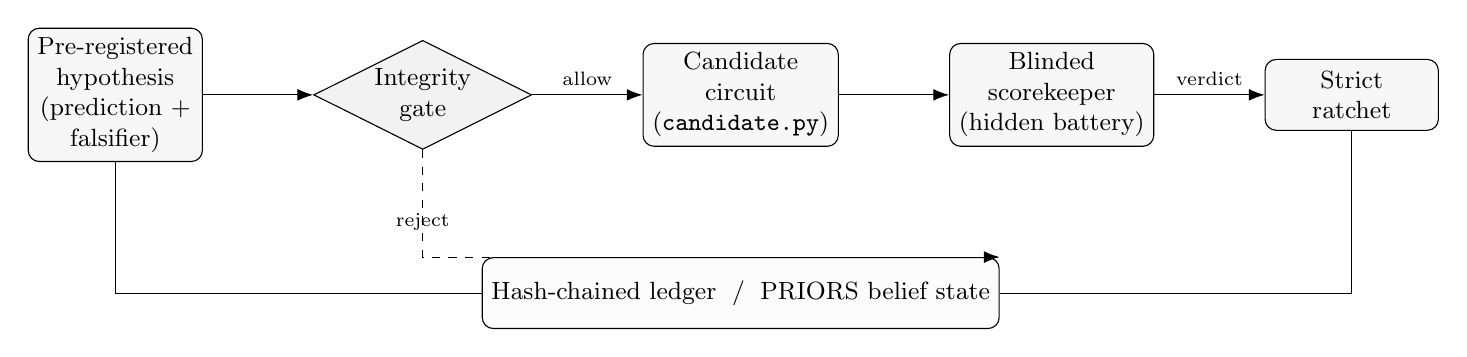
\begin{tikzpicture}[
  node distance=9mm and 14mm,
  box/.style={draw, rounded corners, align=center, minimum height=9mm,
    minimum width=22mm, font=\small, fill=black!3},
  gate/.style={draw, diamond, aspect=2, align=center, font=\small,
    inner sep=1pt, fill=black!5},
  every edge/.style={draw, -{Latex[length=2mm]}},
]
\node[box] (hyp) {Pre-registered\\hypothesis\\(prediction +\\falsifier)};
\node[gate, right=of hyp] (gate) {Integrity\\gate};
\node[box, right=of gate] (impl) {Candidate\\circuit\\(\texttt{candidate.py})};
\node[box, right=of impl] (score) {Blinded\\scorekeeper\\(hidden battery)};
\node[box, right=of score] (ratchet) {Strict\\ratchet};

\draw (hyp) edge (gate);
\draw (gate) edge node[above, font=\scriptsize] {allow} (impl);
\draw (impl) edge (score);
\draw (score) edge node[above, font=\scriptsize] {verdict} (ratchet);

\node[box, below=14mm of impl, fill=black!1] (ledger)
  {Hash-chained ledger \;/\; PRIORS belief state};
\draw (ratchet.south) |- (ledger.east);
\draw (ledger.west) -| (hyp.south);
\draw[dashed, -{Latex[length=2mm]}] (gate.south) |- node[below, pos=0.25,
  font=\scriptsize] {reject} (ledger.north east);
\end{tikzpicture}
\caption{The harness loop for this campaign. A hypothesis is pre-registered with a
falsifier and passes an integrity gate (diff allowlist) before a candidate circuit
is written to the single editable file. A blinded scorekeeper scores it on a hidden
battery; a strict ratchet promotes it only if it is valid and has strictly fewer MS
gates than the incumbent. Every verdict --- promotion, no-improvement, or integrity
rejection --- is written to a hash-chained ledger that updates the belief state and
seeds the next hypothesis. The loop never sees the battery.}
\label{fig:harness}
\end{figure}

\subsection{Scoring metric}

Let $U_{\mathrm{ideal}}$ be the ideal one-Trotter-step unitary (defined below) and
$U_{\mathrm{cand}}$ the unitary implemented by a candidate circuit. For a battery of
input states $\{\psi_i\}$ the state-averaged mean infidelity is
\begin{equation}
\bar{\mathcal{I}} \;=\; \frac{1}{n}\sum_{i=1}^{n}
  \Bigl( 1 - \bigl|\langle U_{\mathrm{ideal}}\psi_i \,|\, U_{\mathrm{cand}}\psi_i
  \rangle\bigr|^{2} \Bigr).
\label{eq:infid}
\end{equation}
The score is
\begin{equation}
\mathrm{Score} \;=\;
\begin{cases}
  \#\{\text{MS gates}\}, & \text{if the circuit is native and }
    \bar{\mathcal{I}} \le 10^{-4},\\[2pt]
  10^{6}, & \text{otherwise (INVALID).}
\end{cases}
\label{eq:score}
\end{equation}
Lower is better. The battery here has $n=48$ states, mixing Haar-random,
random-product, and computational-basis states; the seeds are hidden. Estimating
infidelity on a finite battery, rather than computing the full operator distance
\cite{NielsenChuang2010}, is what keeps the test instances hideable while remaining
a faithful proxy (Section~\ref{sec:discussion}).

\subsection{Why the reference is \texorpdfstring{$U_{\mathrm{ideal}}$}{U\_ideal}, not
\texorpdfstring{$e^{-iH\,\mathrm{d}t}$}{exp(-iH dt)}}
\label{sec:uideal}

$U_{\mathrm{ideal}}$ is the exact ordered product of the block exponentials of one
Trotter step --- the uncompiled ideal circuit of \cite{Srinivasan2024}, denoted
$\hat{C}$ --- applied by statevector simulation. It is \emph{not} the matrix
exponential $e^{-iH\,\mathrm{d}t}$ of the full Hamiltonian. This choice is
load-bearing. At $\mathrm{d}t = 0.3$ the first-order Trotter error between the
product-of-block circuit and $e^{-iH\,\mathrm{d}t}$ is far larger than $10^{-4}$, so
scoring a compiled circuit against $e^{-iH\,\mathrm{d}t}$ with an $\varepsilon =
10^{-4}$ bar would be ill-posed: no native circuit could ever pass, because the
Trotter error alone exceeds the bar. Certifying against $U_{\mathrm{ideal}}$ isolates
the quantity we actually study --- how faithfully a native circuit reproduces the
intended Trotter operator --- and it matches the methodology of
\cite{Srinivasan2024}, whose own random-state check scores the compiled circuit
against the ideal Trotter circuit $\hat{C}$. Fidelity is always certified against
this ideal unitary, never against a noise realization.

\subsection{What the director supplied (seeding disclosure)}
\label{sec:seeding}

Honest reporting of an autonomous loop requires stating exactly what was
human-supplied. Two things were, and we disclose them symmetrically.

\emph{The win recipe.} The public contract handed the loop the target ($9N = 54$),
the per-block MS minimum (4 MS per hopping block), the 12-fold identity of the
hopping blocks, and an IPG-style tool \texttt{fit\_block} that re-optimizes the
continuous angles of an $n$-MS ansatz to match a given block unitary. Reaching 54 MS
was therefore the execution of a fully specified strategy, not a discovery.

\emph{The four attack lanes for beating 54.} The campaign direction --- an organ every
session reads --- additionally enumerated four routes for going strictly below 54:
(1) per-block resynthesis to the 4-MS minimum; (2) whole-circuit angle
re-optimization of a fixed low-MS structure; (3) cross-block merging of
qubit-sharing blocks; and (4) approximate pruning of low-weight MS gates. The three
sub-54 experiments below worked \emph{within} these human-enumerated lanes: the
belief state tags EXP-0002 as lane~4, EXP-0003 as lane~2/3, and EXP-0004 as lane~3.
We do not claim the loop invented these routes.

\emph{What the loop did unaided.} Within the human-supplied lanes, and only within
them, the loop performed the following without further human input, and these are
real: (i) it instantiated each lane as a concrete, runnable 18-qubit circuit
construction; (ii) it wrote a falsifier and a kill-threshold for each; (iii) it
generated a \emph{self-priced chain of reopening conditions} --- each refuted
experiment priced the exact offline probe that the next experiment had to pass
before any submission (EXP-0002 $\to$ EXP-0003 $\to$ EXP-0004) --- which is
genuinely self-generated; (iv) it made the offline feasibility determinations that
decided when \emph{not} to submit (for example the pruning-budget calculation
$k = \lfloor 5\times10^{-5}/r\rfloor = 0$ in EXP-0002); and (v) it extracted the
closing physical mechanism (Section~\ref{sec:discussion}). We frame this as
autonomous falsification, pricing, and mechanism extraction within human-suggested
lanes --- not autonomous hypothesis generation.

\section{Results}
\label{sec:results}

The campaign ran four experiments over four cycles with one promotion. Every number
in Table~\ref{tab:results} is copied from the corresponding blinded verdict JSON;
none is self-reported. The baseline (EXP-0000) is an immutable naive CNOT-ladder
compilation that scores 102 MS. Its verdict logs only validity
($\bar{\mathcal{I}} \le 10^{-4}$) with no recorded exponent, so we report it as
``valid'' rather than quoting a specific infidelity.

\begin{table}[t]
\centering
\small
\begin{tabular}{@{}llrrll@{}}
\toprule
Exp. & Hypothesis (lane) & MS & Mean infidelity & Valid & Gate decision \\
\midrule
EXP-0000 & Baseline (naive ladder)        & 102 & $\le 10^{-4}$           & yes & baseline lock \\
EXP-0001 & Per-block resynthesis (recipe) & 54  & $2.38\times10^{-13}$    & yes & \textbf{promoted} \\
EXP-0002 & Approx.\ pruning (lane 4)      & 54  & $2.38\times10^{-13}$    & yes & no-improvement \\
EXP-0003 & Angle compensation (lane 2/3)  & 53  & $3.13\times10^{-1}$     & no  & rejected (integrity) \\
EXP-0004 & Structural merge (lane 3)      & 54  & $2.38\times10^{-13}$    & yes & no-improvement \\
\bottomrule
\end{tabular}
\caption{The four experiments, verbatim from the blinded verdicts. Score is the MS
count when valid. EXP-0001 is the single promotion: a valid 54-MS circuit at mean
infidelity $2.38\times10^{-13}$, a $(102-54)/102 = 47\%$ reduction against the
baseline in our ruler. EXP-0002 and EXP-0004 determined infeasibility offline and
resubmitted the incumbent (identical infidelity, bit for bit). EXP-0003 submitted a
53-MS circuit that the blinded scorekeeper certified invalid at mean infidelity
$0.313$, so it scored $10^{6}$ and could not promote.}
\label{tab:results}
\end{table}

\begin{figure}[t]
\centering
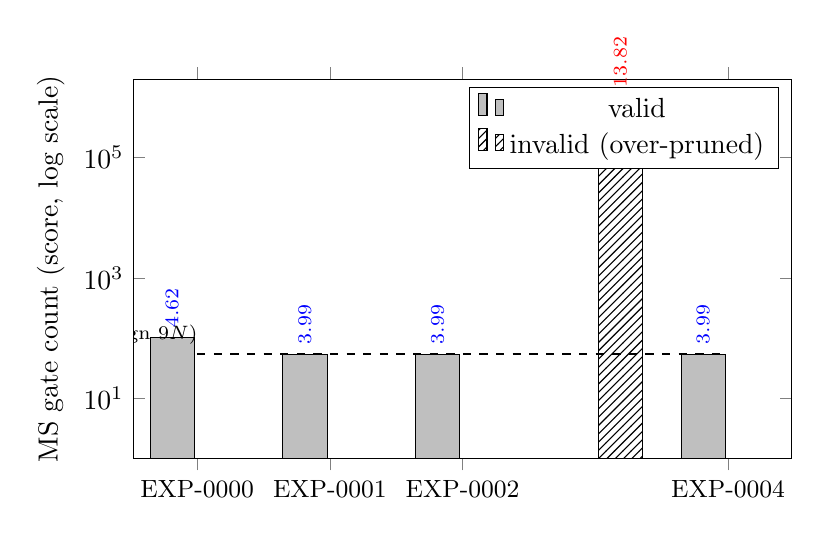
\begin{tikzpicture}
\begin{axis}[
  width=0.82\textwidth, height=6.4cm,
  ybar,
  bar width=16pt,
  ymode=log,
  ymin=1, ymax=2e6,
  ylabel={MS gate count (score, log scale)},
  symbolic x coords={EXP-0000,EXP-0001,EXP-0002,EXP-0003,EXP-0004},
  xtick=data,
  x tick label style={font=\small},
  nodes near coords,
  nodes near coords style={font=\scriptsize},
  every node near coord/.append style={anchor=west, rotate=90},
  enlarge x limits=0.12,
]
\addplot+[draw=black, fill=black!25] coordinates {
  (EXP-0000,102) (EXP-0001,54) (EXP-0002,54) (EXP-0004,54)
};
\addplot+[draw=black, fill=black!55, pattern=north east lines] coordinates {
  (EXP-0003,1000000)
};
\draw[dashed, thick] (axis cs:EXP-0000,54) -- (axis cs:EXP-0004,54)
  node[above left, pos=0.02, font=\scriptsize] {ship bound = 54 (hand design $9N$)};
\legend{valid, invalid (over-pruned)}
\end{axis}
\end{tikzpicture}
\caption{Score per experiment (MS count when valid, $10^{6}$ when invalid), on a log
axis. The baseline sits at 102; the single promotion (EXP-0001) drops to the 54-MS
ship bound and stays there. EXP-0003's 53-MS candidate --- one gate below the bound ---
was certified invalid at mean infidelity $0.313$ and scored $10^{6}$: the blinded
verifier catching an over-pruning that looked plausible from a gate-count view
alone.}
\label{fig:scores}
\end{figure}

\subsection{EXP-0001 --- verification of the hand design (promotion)}

Following the human-specified recipe of Section~\ref{sec:seeding}, the loop fit the
canonical hopping block $U_{\mathrm{hop}}$ to a 4-MS native ansatz once, replicated
it to all 12 hopping blocks by qubit relabelling, and realized each on-site block as
a single MS gate, giving $12\times4 + 6\times1 = 54$ MS
(Eq.~\eqref{eq:count}). The blinded scorekeeper returned a valid circuit at mean
infidelity $2.38\times10^{-13}$ (48-state battery), and the ratchet promoted it from
the 102-MS baseline: a delta of $-48$ MS in a single step. This certifies that the
harness reproduces the hand-designed $9N=54$ endpoint of \cite{Srinivasan2024} at
machine precision. It is verification of a supplied strategy, not autonomous
rediscovery. We report the reduction in our own ruler as $102\to54$, i.e.\ 47\%;
the 36\% figure ($84\to54$) is Srinivasan's, measured in Srinivasan's direct-native
ruler, which we do \emph{not} reproduce (our baseline is a different naive
compilation at 102 MS).

\subsection{EXP-0002 through EXP-0004 --- the honest null below 54}

Each sub-54 experiment attacked a distinct human-enumerated lane, and each closed
its predecessor's priced door.

\emph{EXP-0002 (lane 4, approximate pruning).} Prediction: if the best 3-MS fit of a
hopping block has residual infidelity $r$, then because block errors add roughly
linearly one can prune $k = \lfloor 5\times10^{-5}/r \rfloor$ of the 12 hopping
blocks from 4 to 3 MS and stay under the bar, yielding a $(54-k)$-MS circuit.
Falsifier: if $r > 5\times10^{-5}$ then $k=0$ and not even one block can be pruned.
The loop's own offline analysis found $r > 5\times10^{-5}$, so $k=0$; it therefore
resubmitted the 54-MS incumbent, which the scorekeeper scored valid at the identical
$2.38\times10^{-13}$ (delta $0$, no improvement). This determination was made offline
--- the loop declined to spend a submission on a circuit it had already shown could not
beat 54. It priced the next door: reopen only if a \emph{whole-circuit} angle
optimizer over a fixed 53-MS ansatz shows $\bar{\mathcal{I}}\le10^{-4}$ is feasible.

\emph{EXP-0003 (lane 2/3, angle compensation) --- the one blinded refutation.} The loop
removed the 4th MS of one hopping block and jointly re-optimized, by L-BFGS, the
native angles of that block's 3-MS ansatz together with every block sharing its
qubits, hoping neighbours could compensate the missing entangler. This is the one
sub-54 circuit actually submitted: a 53-MS candidate. The blinded scorekeeper
certified it INVALID at mean infidelity $0.313$ --- five thousand times over the bar
--- so it scored $10^{6}$ (gate decision: rejected on integrity, delta $+999946$).
This is the harness catching a plausible-looking over-pruning, the failure mode
raised against the learned-Hamiltonian experiment of \cite{Jafferis2022}: a
gate-count view alone would have called this a win.

\emph{EXP-0004 (lane 3, structural merging).} The loop enumerated the frozen block
order for a consecutive pair of hopping blocks sharing a qubit with no intervening
block on their combined support, formed the joint 5-qubit unitary, and probed
whether it compresses $8\to7$ MS at the fidelity bar. Its offline probe showed no
qualifying pair reaches $\bar{\mathcal{I}}\le10^{-4}$ at 53 MS; it resubmitted the
54-MS incumbent (valid, $2.38\times10^{-13}$, no improvement) and priced the next
door (a strictly larger exact structural unit). With three consecutive
non-promotions, the kill criterion fired and the search consolidated.

\subsection{Provenance}

Across the run: 4 experiments, 1 promotion, 1 integrity rejection, 0 crashes, and 0
hash-chain breaks. The dataset source is SEALED on every scored row, and the
scorekeeper build was held constant (0 rows measured under a different scorer build
than the baseline). The per-row harness commit hashes differ because the repository
HEAD advances on every mutation; the scoring code did not change
(Section~\ref{sec:code}).

\section{Discussion}
\label{sec:discussion}

\paragraph{The mechanism the loop extracted.} The three refutations share one cause,
which the loop stated explicitly at close: the 4th MS gate of a hopping block carries
irreducible two-qubit entangling content, and that content cannot be manufactured by
the free single-qubit angles (GPi, GPi2, RZ) of neighbouring blocks. Joining two
blocks at a shared qubit only stitches their supports together; it does not let one
block's entangling budget pay for another's. In one phrase: \emph{MS entangling power
is conserved, not fungible}. This is why per-block pruning (EXP-0002), angle
compensation (EXP-0003), and structural merging (EXP-0004) all fail to reach 53 MS at
the bar, and it is consistent with the per-block minimum of 4 MS being genuinely
exact. Extracting this mechanism from three refutations --- rather than continuing to
spend submissions --- is the substantive autonomous act in the campaign.

\paragraph{Why the finite battery is trustworthy.} One might worry that passing a
48-state battery over-fits to a lucky input distribution --- exactly the over-pruning
failure raised against the learned-Hamiltonian experiment of \cite{Jafferis2022},
where a circuit tuned to a specific realization looked faithful and was not. Two
facts guard against it here. First, fidelity is certified against the ideal unitary
$U_{\mathrm{ideal}}$, never against a noise realization. Second, the battery includes
Haar-random states in the full $d = 2^{18}$ Hilbert space, where inner products
concentrate sharply; a circuit that passes $10^{-4}$ mean infidelity on such states
strongly evidences genuine operator-level fidelity rather than distributional
over-fitting. (The concentration argument applies strictly to the Haar component of
the mixed battery; see Limitations.) The EXP-0001 promotion at $2.38\times10^{-13}$
--- nine orders below the bar --- is not a near-threshold pass that could be an artifact
of the battery.

\paragraph{What the result is.} The load-bearing contribution is the harness, not a
circuit. An integrity-gated, pre-registered system took a real published result,
faithfully executed a human-specified compression down to the hand-designed $9N=54$
optimum, and had a blinded, independent verifier certify it at machine precision with
a full hash-chained audit trail and nothing self-reported. The same verifier then
caught a plausible 53-MS over-pruning, and the loop reached an honest null on the
open question beyond the target without overclaiming. That combination --- reproduce,
self-certify, refuse to fool itself --- is the collaboration proof the campaign was
built to produce.

\section{Limitations}
\label{sec:limitations}

\begin{itemize}
\item \emph{Scope.} This is one first-order Trotter step, at one parameter point
($J=1$, $U=2$, $\mathrm{d}t=0.3$), for $N=6$. It is a classical statevector
replication of one circuit-compression claim; it uses no quantum hardware and does
not reproduce the physics results of \cite{Srinivasan2024}.
\item \emph{Ruler.} The 47\% reduction is measured against our own 102-MS naive
baseline, not against Srinivasan's $14N=84$ direct compilation. We reproduce the
hand-designed 54-MS \emph{endpoint} at machine precision; we do not reproduce the
36\% figure, which lives in Srinivasan's ruler.
\item \emph{Not a suboptimality claim.} 54 MS is a firm bound only within this ruler
and this $10^{-4}$ fidelity bar. We refute three specific sub-54 routes; we do
\emph{not} prove no sub-54 circuit exists, and we do not claim the hand design is
suboptimal.
\item \emph{Autonomy.} The win recipe and all four sub-54 attack lanes were
human-supplied. The loop's unaided contribution is limited to instantiation,
falsifier writing, priced reopening, offline feasibility determination, and
mechanism extraction within those lanes (Section~\ref{sec:seeding}).
\item \emph{Battery.} Infidelity is estimated on a finite hidden battery of 48
states; the Haar-concentration argument applies strictly to the Haar component of the
mixed battery. A larger or differently constructed battery could in principle change a
near-threshold verdict, though not the machine-precision EXP-0001 result.
\end{itemize}

\section{AI-contribution statement}
\label{sec:ai}

The authors are solely responsible for this paper's claims, framing, and
conclusions. The research ran inside an autonomous multi-agent harness in which
AI agents proposed hypotheses, wrote candidate circuits, and drafted this manuscript;
an independent blinded scorekeeper produced every score, and no number in this paper
is self-reported by an agent. Each hypothesis was pre-registered with a falsifier
before execution, and the draft was subjected to an adversarial critic panel before
release. The human authors verified the reported numbers against the blinded verdict
records, checked the bibliography entry-by-entry against the primary sources, and are
accountable for the honest-null framing and the seeding disclosures. AI systems are
not authors; this statement is a methods disclosure, provided because undisclosed AI
authorship or AI-generated content is grounds for rejection at scientific venues.

\section{Code and data availability}
\label{sec:code}

The reproduction repository is
\url{https://github.com/oharalabsai/dhruv-fhm-gate-search-repro}. It contains the
final 54-MS candidate circuit, every scored candidate with its blinded verdict JSON,
the frozen public contract and target module (Hamiltonian, native-gate matrices,
$U_{\mathrm{ideal}}$, and the self-check tool), and the append-only ledger and belief
state. The scoring battery seeds remain sealed by design. Note that the per-experiment
harness commit hashes recorded in the verdicts differ because the repository HEAD
advances on every mutation of the ledger; the scoring code itself was held constant
across the run (0 rows were measured under a different scorer build than the
baseline).

\bibliographystyle{unsrt}
\bibliography{references}

\end{document}
